\documentclass{article}
\usepackage[T1]{fontenc}
\usepackage[utf8]{inputenc}
\usepackage{lmodern}
\usepackage[ngerman]{babel}
\usepackage{amsmath, amssymb}
\usepackage{array}
\usepackage{phonetic} % for reversed D
\usepackage{wasysym}  % for the notes
\usepackage{tikz, tikzsymbols}
\usepackage{xcolor}
\usetikzlibrary{arrows,automata,fit}
\setlength\parindent{0pt}

\newcommand{\rpt}{%
        \raisebox{.2ex}{:}%
        \raisebox{-.4ex}{\rule{.1ex}{2.5ex}\,\rule{.2ex}{2.5ex}}}
\newcommand{\revrpt}{%
        \raisebox{-.2ex}{\rule{.2ex}{2.5ex}\,\rule{.1ex}{2.5ex}}%
        \raisebox{.2ex}{:}}
    
\begin{document}

\begin{center}
  \Large{Informatik \revD: Übungsblatt 7}

  \large{Sebastian Höffner, Andrea Suckro}
\end{center}



\section*{Aufgabe 7.1}
\section*{Aufgabe 7.2}
\section*{Aufgabe 7.3}
\subsection*{Leerheitsproblem}
\begin{center}
Initial:\\
\begin{tabular}{ll}
$S \rightarrow E | ABC$               & $A \rightarrow bDC | E | S$ \\
$B \rightarrow acDC | C$              & $C \rightarrow ab | Ja | IdA$ \\
$D \rightarrow deF | DeF | dEF | DEF$ & $E \rightarrow abba | aBBa | AbbA$ \\
$F \rightarrow JcJ | GJ | bG$         & $G \rightarrow F | IG$ \\
$H \rightarrow SA | Hcc$              & $I \rightarrow c | cIc | dF$
\end{tabular}\\
Erster Schritt:\\
\begin{tabular}{ll}
$S \rightarrow {\color{red}E} | AB{\color{red}C}$               & $A \rightarrow bD{\color{red}C} | {\color{red}E} | S$ \\
$B \rightarrow acD{\color{red}C} | {\color{red}C}$              & ${\color{red}C} \rightarrow ab | Ja | {\color{red}I}dA$ \\
$D \rightarrow deF | DeF | d{\color{red}E}F | D{\color{red}E}F$ & ${\color{red}E} \rightarrow abba | aBBa | AbbA$ \\
$F \rightarrow JcJ | GJ | bG$                                   & $G \rightarrow F | {\color{red}I}G$ \\
$H \rightarrow SA | Hcc$                                        & ${\color{red}I} \rightarrow c | c{\color{red}I}c | dF$
\end{tabular}\\
Zweiter Schritt:\\
\begin{tabular}{ll}
${\color{red}S} \rightarrow {\color{red}E} | {\color{red}ABC}$  & ${\color{red}A} \rightarrow bD{\color{red}C} | {\color{red}E} | {\color{red}S}$ \\
${\color{red}B} \rightarrow acD{\color{red}C} | {\color{red}C}$ & ${\color{red}C} \rightarrow ab | Ja | {\color{red}I}d{\color{red}A}$ \\
$D \rightarrow deF | DeF | d{\color{red}E}F | D{\color{red}E}F$ & ${\color{red}E} \rightarrow abba | a{\color{red}BB}a | {\color{red}A}bb{\color{red}A}$ \\
$F \rightarrow JcJ | GJ | bG$                                   & $G \rightarrow F | {\color{red}I}G$ \\
$H \rightarrow {\color{red}SA} | Hcc$                           & ${\color{red}I} \rightarrow c | c{\color{red}I}c | dF$
\end{tabular}
\end{center}
Bereits im zweiten Schritt wird $S$ markiert, also ist $L(G) \neq \emptyset$.

\subsection*{Endlichkeitsproblem}
Wir führen den Algorithmus von oben vorerst zu Ende.
\begin{center}
Dritter Schritt:\\
\begin{tabular}{ll}
${\color{red}S} \rightarrow {\color{red}E} | {\color{red}ABC}$  & ${\color{red}A} \rightarrow bD{\color{red}C} | {\color{red}E} | {\color{red}S}$ \\
${\color{red}B} \rightarrow acD{\color{red}C} | {\color{red}C}$ & ${\color{red}C} \rightarrow ab | Ja | {\color{red}I}d{\color{red}A}$ \\
$D \rightarrow deF | DeF | d{\color{red}E}F | D{\color{red}E}F$ & ${\color{red}E} \rightarrow abba | a{\color{red}BB}a | {\color{red}A}bb{\color{red}A}$ \\
$F \rightarrow JcJ | GJ | bG$                                   & $G \rightarrow F | {\color{red}I}G$ \\
${\color{red}H} \rightarrow {\color{red}SA} | {\color{red}H}cc$ & ${\color{red}I} \rightarrow c | c{\color{red}I}c | dF$
\end{tabular}
\end{center}
Weiter lässt sich nichts markieren, d.h. wir können die Grammatik nun auf die markierten Regeln reduzieren.
\begin{center}
\begin{tabular}{ll}
$S \rightarrow E | ABC$            & $A \rightarrow E | S$ \\
$B \rightarrow C$                  & $C \rightarrow ab | IdA$ \\
$E \rightarrow abba | aBBa | AbbA$ & $H \rightarrow SA | Hcc$ \\
$I \rightarrow c | cIc$            & \\
\end{tabular}
\end{center}
Als nächstes reduzieren wir die Grammatik auf erreichbare Regeln.
\begin{center}
\begin{tabular}{ll}
${\color{red}S} \rightarrow {\color{red}E} | {\color{red}ABC}$                         & ${\color{red}A} \rightarrow {\color{red}E} | {\color{red}S}$ \\
${\color{red}B} \rightarrow {\color{red}C}$                                            & ${\color{red}C} \rightarrow ab | {\color{red}IdA}$ \\
${\color{red}E} \rightarrow abba | a{\color{red}BB}a | {\color{red}A}bb{\color{red}A}$ & $H \rightarrow SA | Hcc$ \\
${\color{red}I} \rightarrow c | c{\color{red}I}c$                                      & \\
\end{tabular}
\end{center}
Übrig bleiben:
\begin{center}
\begin{tabular}{ll}
$S \rightarrow E | ABC$            & $A \rightarrow E | S$ \\
$B \rightarrow C$                  & $C \rightarrow ab | IdA$ \\
$E \rightarrow abba | aBBa | AbbA$ & $I \rightarrow c | cIc$ \\
\end{tabular}
\end{center}
Die Regeln $S \rightarrow E$, $A \rightarrow E$, $A \rightarrow S$ und $B \rightarrow C$ müssen transformiert werden. Die transformierte Grammatik sieht z.B. so aus:
\begin{center}
\begin{tabular}{ll}
$S \rightarrow abba | aBBa | AbbA | ABC$ & $A \rightarrow abba | aBBa | AbbA | ABC$ \\
$B \rightarrow ab | IdA$                 & $C \rightarrow ab | IdA$ \\
$E \rightarrow abba | AbbA | aBBa$       & $I \rightarrow c | cIc$ \\
\end{tabular}
\end{center}

Wir erstellen einen Hilfsgraph auf Grundlage der reduzierten und vereinfachten Grammatik.
\begin{center}
\begin{tikzpicture}[->, auto, node distance=2cm]
  \node[state] (S)                   {$S$};
  \node[state] (A) [right of=S]      {$A$};
  \node[state] (B) [below of=S]      {$B$};
  \node[state] (C) [above of=S] {$C$};
  \node[state] (E) [right of=B]      {$E$}; 
  \node[state] (I) [left of=S] {$I$};

  \path (S) edge node {} (A)
            edge node {} (B)
            edge node {} (C)
        (A) edge [bend left] node {} (B)
            edge [bend left] node {} (C)
            edge [loop right] node {} (A)
        (B) edge [bend left] node {} (A)
            edge node {} (I)
        (C) edge [bend left] node {} (A)
            edge node {} (I)
        (E) edge node {} (A)
            edge node {} (B)
        (I) edge [loop below] node {} (I)    
        ;
\end{tikzpicture}
\end{center}

Es gibt gerichtete Kreise $B \leftrightarrow A \leftrightarrow C$, sowie $A$ und $I$ auf sich selbst. Somit ist $|L(G)| = \infty$.

\section*{Aufgabe 7.4}

\newpage

\section*{Aufgabe 7.5}
\begin{figure}[h]
  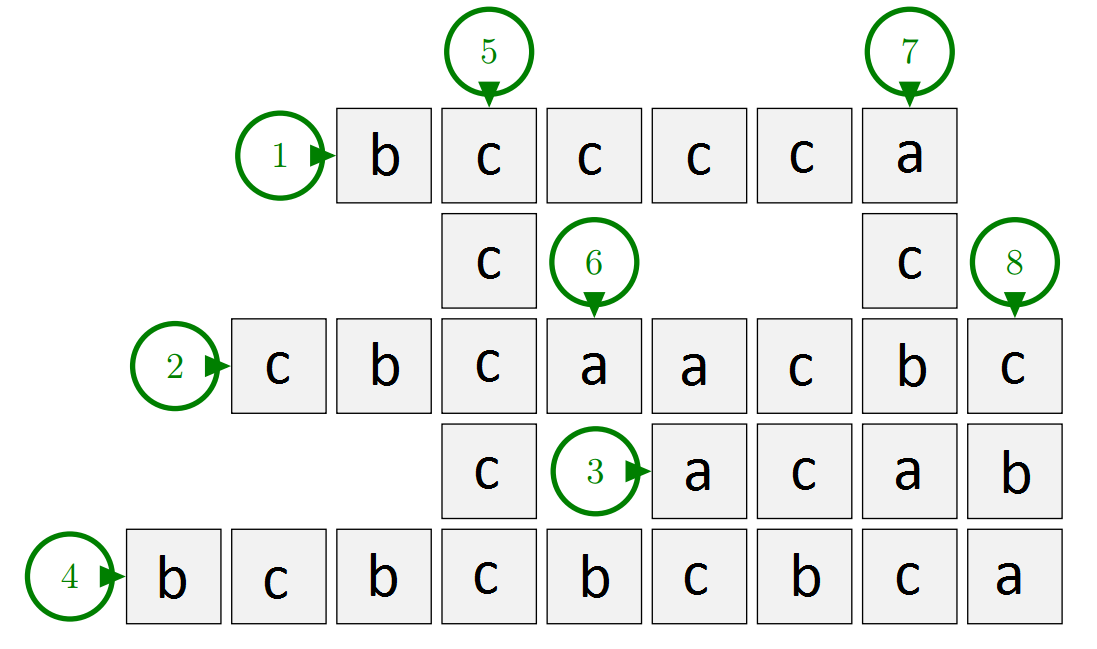
\includegraphics[scale=0.4]{crossword.png}
\end{figure}


\section*{Aufgabe 7.6}
Es war einmal ein armes, frommes Mädchen, das lebte mit seiner Mutter allein, und sie hatten nichts mehr zu essen. Da ging das Kind hinaus in den Wald, und begegnete ihm da eine alte Frau, die wusste seinen Jammer schon und schenkte ihm ein Töpfchen, zu dem sollt es sagen: "Töpfchen, koche," so kochte es guten, süssen Hirsebrei, und wenn es sagte: "Töpfchen, steh," so hörte es wieder auf zu kochen.

Das Mädchen brachte den Topf seiner Mutter heim, und nun waren sie ihrer Armut und ihres Hungers ledig und assen süssen Brei, sooft sie wollten.

Auf eine Zeit war das Mädchen ausgegangen, da sprach die Mutter: "Töpfchen, koche," da kocht es, und sie isst sich satt; nun will sie, dass das Töpfchen wieder aufhören soll, aber sie weiss das Wort nicht. Also kocht es fort, und der Brei steigt über den Rand hinaus und kocht immerzu, die Küche und das ganze Haus voll und das zweite Haus und dann die Strasse, als wollt's die ganze Welt satt machen, und ist die grösste Not, und kein Mensch weiss sich da zu helfen. Endlich, wie nur noch ein einziges Haus übrig ist, da kommt das Kind heim und spricht nur: "Töpfchen, steh," da steht es und hört auf zu kochen, und wer wieder in die Stadt wollte, der musste sich durchessen.


\end{document}
